In this section, we treat the domain parameterization using the \emph{mapping approach}.
First, we will introduce the method in Section~\ref{subsubsec:mapping-approach}.
Afterward, we will apply the mapping approach to the variational formulations of the Poisson and Helmholtz equations in Sections~\ref{subsubsec:poisson-mapping} and~\ref{subsubsec:helmholtz-mapping}.

\subsection{General description}\label{subsubsec:mapping-approach}
We model the parameterized domain as a deformation of a Lipschitz reference domain, which we denote as ${D}$ for both the interior Poisson domain and the exterior Helmholtz scattering domain.
In the spirit of~\cite{castrillon-candas2016,harbrecht2016,hiptmair2018}, we apply a mapping approach~\cite{tartakovsky2006,xiu2006} to pull the variational formulation defined on ${D}(\y)$ back onto the reference domain ${D}$ using a parameter-dependent diffeomorphism $\Phi(\y) :{D} \to {D}(\y)$, $\y\in Y$.
Such technique is often used in shape optimization~\cite{haubner2021,haubner2020,hiptmair2015,onyshkevych2021} and provides a framework for which theory and discretization algorithms are well established.
Following~\cite{cohen2018}, and motivated by similar approaches in shape optimization~\cite{haubner2020}, we consider maps that depend affinely on the entries of $\y$:
\begin{equation}
    \Phi(\y; \x) = \x + \sum_{j\geq 1} \Phi_j({\bm{x}})y_j,\quad \x \in {D}.\label{eq:phidefpois}
\end{equation}
In the uncertainty quantification framework, one could arrive at this representation by considering it as a vector-valued version of the Kar\-hun\-en-\-Loève expansion; see, for example,~\cite{harbrecht2016}.
However,~\eqref{eq:phidefpois} could also be a parametric representation used, for instance, for optimization purposes~\cite{hicks1978,martins2022,hiptmair2015}.

Other approaches different from the mapping approach are possible to handle parameter-dependent geometries.
The fictitious domain approach~\cite{canuto2007} and level set methods~\cite{nouy2008,nouy2007, osher2001} embed the parameter-dependent domain in a larger, hold-all domain, and level set methods can handle both geometrical and topological changes.
However, since these techniques recast a problem on a parameter-dependent domain to a problem with a parametric interface, the issue raised in~\cite{motamed2013,scarabosio2017,scarabosio2022} appears.
Namely, the solution depends non-smoothly on the parameter in a neighborhood of the boundary, affecting the convergence of algorithms for polynomial-based surrogates.
In uncertainty quantification, when one is not interested in the surrogate, but in moments of the quantities of interest only, and when the shape variations are small, it is possible to adopt perturbation methods~\cite{dambrine2016,harbrecht2013,harbrecht2008}.

For the map~\eqref{eq:phidefpois}, we formulate the following assumption, which will be used to ensure the well-posedness of the variational formulations:
\begin{assumption}\label{ass:phijpois}
The mapping sequence $(\Phi_j)_{j\geq 1}$ satisfies the following smoothness and decay properties:
\begin{itemize}
    \item we have
    \begin{equation*}
        \Phi(\y;\cdot),  \Phi_j(\cdot)\in W^{1, \infty}(D),\text{ for all }j \geq 1,
    \end{equation*}
    and
    \begin{equation*}
        \Phi^{-1}(\y;\cdot) \in W^{1, \infty}({D}(\y)),\text{ for all }\y \in Y.
    \end{equation*}
    \item there exist constants $C_\Phi, C_{\Phi^{-1}}$, independent of $\y \in Y$, such that we have the bounds
    \begin{equation*}
        \|\Phi(\y;\cdot)\|_{ W^{1, \infty}(D)}< C_\Phi,
    \end{equation*}
    and
    \begin{equation*}
        \|\Phi^{-1}(\y;\cdot)\|_{W^{1, \infty}({D}(\y))} < C_{\Phi^{-1}},
    \end{equation*}
    for all $\y \in Y$.
\end{itemize}
\end{assumption}
We can take derivatives of the mapping $\Phi(\y,\x)$ to obtain the Jacobian matrix $\D\Phi(\y;\x)$.
As a consequence of the Courant-Fisher theorem for singular values~\cite[Thm. 3.1.2]{horn1991}, applied to $\D\Phi(\y)$ and $\D\Phi^{-1}(\y)$, we have:
\begin{lemma} \label{lem:courantfish2pois}
Let Assumption~\ref{ass:phijpois} hold.
We have that, for the singular values of $\D\Phi^{-1}(\y)$, $\sigma_1=\sigma_1(\y; \x), \ldots, \sigma_d=\sigma_d(\y; \x)$, there exist constants $\sigma_{\min},  \sigma_{\max} > 0$, independent of $\y \in Y$, such that
\begin{equation*}
    \sigma_{\min} \leq \sigma_1(\y; \x), \ldots, \sigma_d(\y; \x) \leq \sigma_{\max},
\end{equation*}
for a.e. $\x\in {D}(\y)$ and for all $\y \in Y$.
\end{lemma}

\begin{figure}
    \centering
    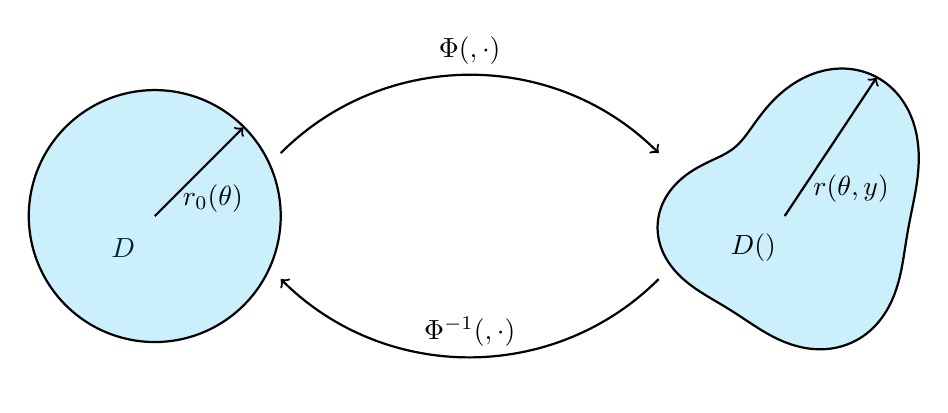
\begin{tikzpicture}[thick, scale=1.6]
        %\draw[domain=0:2*pi,samples=500,dashed,very thin,shift={(3,0)}] plot ({deg(\x)}:{1});
        \draw[fill=cyan,domain=0:3*pi,samples=500,fill opacity=0.2,shift={(3,0)}] plot ({deg(\x)}:{((cos(\x * 1 r)^3 - cos(\x * 3 r) + sin(\x*2 r)*0.5)*0.2+1)});
        \draw[-to,shift={(3,0)}] (0,0) -- (0.73, 1.1) node [pos=0.2, right] {$r(\theta,\bm{y})$};
        %\draw[-to, dashed,shift={(3,0)}] (0,0) -- (-0.703, 0.703) node [pos=0.2, left] {$r_0(\theta)\,\,$};
        \draw[->, thick] (-1,0.5) to [bend left=45]  node [above,pos=0.5] {$\Phi(\y, \cdot)$} (2,0.5);
        \draw[<-, thick] (-1,-0.5) to [bend right=45]  node [above,pos=0.5] {$\Phi^{-1}(\y, \cdot)$} (2,-0.5);
        \node at (-2.25,-0.25) {${D}$};
        \node at (2.75,-0.25) {$D(\y)$};
        \draw[fill=cyan,domain=0:3*pi,samples=500,fill opacity=0.2,shift={(-2,0)}] plot ({deg(\x)}:{1});
        \draw[-to,shift={(-2,0)}] (0,0) -- (0.703, 0.703) node [pos=0.2, right] {$r_0(\theta)$};
    \end{tikzpicture}
    \caption{Schematic overview of the mapping approach with an interior domain. The domain on the left is the reference domain, with the parameter-dependent mapping $\Phi(\y, \cdot)$ from the reference domain to the parameterized domain.}
    \label{fig:mappingappraochtikz}
\end{figure}
Figure~\ref{fig:mappingappraochtikz} shows a schematic sketch of the mapping approach for the interior domain.

In this section, we started with a radius expansion and used it to define a mapping.
Instead, one can model the shape variations directly, omitting the intermediate radius expansion.
However, we do not consider this approach further in this thesis.

\subsubsection{Poisson equation}\label{subsubsec:poisson-mapping}
With the mapping $\Phi(\y; \x)$ at hand, we can write the following variational problem on the reference domain:

For every $\y\in Y$, find $u(\y) \in V$ such that,
\begin{align}
    &\int_{{D}} {A}(\y) {\nabla} {u}(\y) \cdot  {\nabla} {v} \d\x = \int_{{D}} F(\y) {v} \dx, \label{eq:transformedvarformpois}
\end{align}
for all $v \in V$ where $V\coloneqq H_0^1(D)$,
\begin{align}
{A}(\y; \x) \coloneqq (a\circ\Phi(\y; \x)) \D\Phi^{-1}&(\y; \x) \nonumber\\\D\Phi^{-\top}(\y; \x)
&\det(\D\Phi(\y; \x)), \label{eq:hatAdefpois}
\end{align}
and
\begin{align}
    F(\y; \x) \coloneqq (f\circ\Phi(\y; \x)) \det(\D\Phi(\y; \x)).\label{eq:hatfdefpois}
\end{align}
Under Assumptions~\ref{ass:analytic} and~\ref{ass:phijpois}, the problem~\eqref{eq:transformedvarformpois} is well-posed and $\|u(\y)\|_{V}$ has an $y$-independent upper bound.

From equation~\eqref{eq:transformedvarformpois}, we can see that the shape problem, together with the mapping approach, constitutes an example of the parameterized heterogeneous Poisson equation~\eqref{eq:varformpoisson}.


\subsubsection{Helmholtz equation}\label{subsubsec:helmholtz-mapping}
Similar to the Poisson equation, we pull the variational form~\eqref{eq:varformhelmholtz_shape} back to the reference domain using the mapping~\eqref{eq:phidefpois}.
With this, we arrive at the variational problem:

For every $\y\in Y$, find $u(\y) \in V$ such that,
\begin{align}
    \int_D A(\y) \nabla u(\y) \cdot \nabla v \dx &-k^2\int_D n(\y)  u(\y) v \dx -ik\int_{\Gamma_{out}} u(\y) v \dx \nonumber\\
    &= \int_{\Gamma_{out}} \left( \frac{\partial}{\partial\bm{n}} -ik\right) u_{in} v \dx,\label{eq:varformhelmholtzshape}
\end{align}
for all $\y\in Y$ where $V\coloneqq H_0^1(D)$, $A(\y; \x)$ is defined as in~\eqref{eq:hatAdefpois} with $a_{out}$ instead of $a$ and
\begin{equation*}
    n(\y, \x) = n_{out}\circ\det(\D\Phi(\y; \x)).
\end{equation*}
Clearly, this is a specific instance of the parameterized exterior Helmholtz scattering problem~\eqref{eq:varformhelmholtz}.

There are several mappings to be explored, and we introduce two: a mollifier approach and a harmonic mapping approach, which serves as a prototype for PDE-based mappings.
